% Requires \usepackage{tikz}. No TikZ libraries are required.
\begin{figure}[t]
  \centering
  \resizebox{\columnwidth}{!}{%
  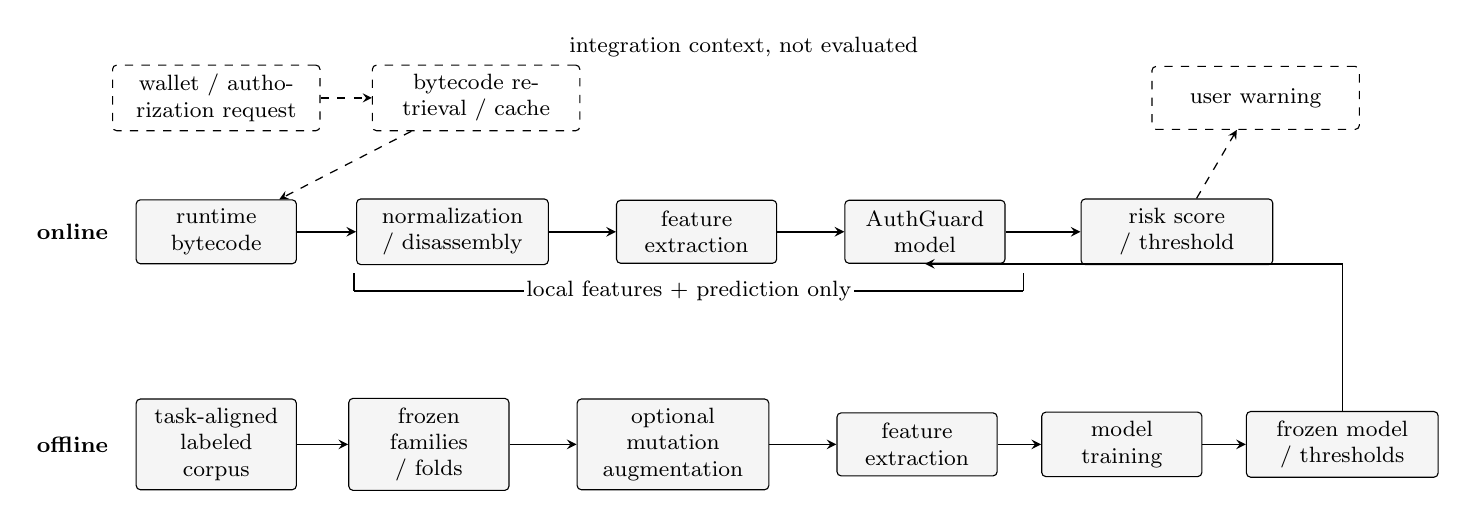
\begin{tikzpicture}[
      font=\footnotesize,
      box/.style={draw=black, rounded corners=1.5pt, minimum height=8mm,
                  text width=22mm, align=center, fill=gray!8},
      smallbox/.style={draw=black, rounded corners=1.5pt, minimum height=8mm,
                       text width=18mm, align=center, fill=gray!8},
      ext/.style={draw=black, dashed, rounded corners=1.5pt, minimum height=8mm,
                  text width=24mm, align=center, fill=white},
      flow/.style={draw=black, ->, >=stealth, line width=.55pt},
      context/.style={draw=black, dashed, ->, >=stealth, line width=.45pt}
    ]
    % External integration context.
    \node[ext] (request) at (0,5.6) {wallet / authorization request};
    \node[ext] (retrieve) at (3.3,5.6) {bytecode retrieval / cache};
    \node[ext] (warning) at (13.2,5.6) {user warning};
    \draw[context] (request) -- (retrieve);
    \node[align=center] at (6.7,6.25) {integration context, not evaluated};

    % Implemented online scorer.
    \node[smallbox] (runtime) at (0,3.9) {runtime bytecode};
    \node[box] (norm) at (3.0,3.9) {normalization / disassembly};
    \node[smallbox] (features) at (6.1,3.9) {feature extraction};
    \node[smallbox] (model) at (9.0,3.9) {AuthGuard model};
    \node[box] (decision) at (12.2,3.9) {risk score / threshold};
    \draw[context] (retrieve) -- (runtime);
    \draw[flow] (runtime) -- (norm);
    \draw[flow] (norm) -- (features);
    \draw[flow] (features) -- (model);
    \draw[flow] (model) -- (decision);
    \draw[context] (decision) -- (warning);
    \node[anchor=east] at (-1.25,3.9) {\textbf{online}};

    % Timing boundary (normalization/disassembly is part of feature construction).
    \draw[line width=.5pt] (1.75,3.15) -- (10.25,3.15);
    \draw[line width=.5pt] (1.75,3.15) -- (1.75,3.38);
    \draw[line width=.5pt] (10.25,3.15) -- (10.25,3.38);
    \node[fill=white, inner sep=1pt] at (6.0,3.15)
      {local features + prediction only};

    % Implemented offline fitting path.
    \node[smallbox] (corpus) at (0,1.2) {task-aligned labeled corpus};
    \node[smallbox] (folds) at (2.7,1.2) {frozen families / folds};
    \node[box] (augment) at (5.8,1.2) {optional mutation augmentation};
    \node[smallbox] (offfeat) at (8.9,1.2) {feature extraction};
    \node[smallbox] (training) at (11.5,1.2) {model training};
    \node[box] (frozen) at (14.3,1.2) {frozen model / thresholds};
    \draw[flow] (corpus) -- (folds);
    \draw[flow] (folds) -- (augment);
    \draw[flow] (augment) -- (offfeat);
    \draw[flow] (offfeat) -- (training);
    \draw[flow] (training) -- (frozen);
    \draw[flow] (frozen.north) |- (model.south);
    \node[anchor=east] at (-1.25,1.2) {\textbf{offline}};
  \end{tikzpicture}%
  }
  \caption{AuthGuard-7702 architecture. Solid nodes are implemented scorer and training paths; dashed nodes and arrows are integration context, not evaluated. The timing boundary covers only local feature construction and prediction.}
  \label{fig:system-architecture}
\end{figure}
